%% The openany option is here just to remove the blank pages before a new chapter
%\documentclass[11pt,openany]{book}
\documentclass[11pt, fleqn]{article}


\usepackage{fullpage}
\usepackage{pagenote}

%%%%%%%%%%%%% For customising the endnote markers. Comment these out if you don't want them.
% To prefix each note number with the chapter number
\renewcommand{\thepagenote}{\thechapter-\arabic{pagenote}}

% To have a slightly different formatting for the endnote numbers in the text -- smaller text, sans-serif, square brackets
\renewcommand\notenumintext[1]{\space{\footnotesize\sffamily[FN-#1]}}

% To have a slightly different formatting for the endnote numbers in the notes section. Just the square brackets and sans-serif; normal size.
\renewcommand\notenuminnotes[1]{{\sffamily[FN-#1] }}

% If you want a different name/heading for the end notes
\renewcommand{\notesname}{End Notes}
%%%%%%%%%%%%% End customisation


%% THIS LINE IS MANDATORY
\makepagenote

\usepackage{hyperref}
\usepackage{minted}
\usepackage{graphicx}
\usepackage{float}

\graphicspath{img/}


\title{{\Huge \textbf{TensorFlow}}\vspace{-1cm}}
\date{}
\maketitle

\begin{document}
%\section{Introduction}

\section{Tensorflow}
TensorFlow is a framework for numerical computation using data flow graphs. Nodes in the graph represent mathematical operations (e.g. sum), and the graph edges represent the multidimensional data arrays (tensors) communicated between them. This architecture gives flexibility to process some nodes on a GPU and others on a CPU, or process the graph in a cluster.

%For example, if we want sum two constants using TensorFlow:
A simple example of an use of Tensorflow is shown below. This example performs a computation that adds two constants (node1 and node2)  and stores the result into node3. Executing this example gives 7.0 as result.

\begin{minted}{python}
node1 = tf.constant(3.0, dtype=tf.float32)
node2 = tf.constant(4.0)
node3 = tf.add(node1, node2)

sess = tf.Session()
print(sess.run(node3))
\end{minted}

During the computation of the example shown above, the following steps are taken: First, a TensorFlow Graph (TFG) is built from the nodes as shown the Figure \ref{fig:TFG_simple}. After that, it is created a session that encapsulates the control and state of the TensorFlow runtime. Finally, the command run is invoked in order to execute the TFG built. 

\begin{figure}[!htp]
    \centering
    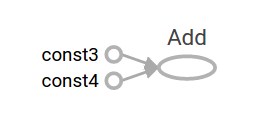
\includegraphics[width=0.4\textwidth]{img/const_add.png}
    \caption{TensorFlow Graph example}
    \label{fig:TFG_simple}
\end{figure}

\subsection{Tensors}
The central unit of data in TensorFlow is the tensor. A tensor consists of a set of primitive values shaped into an array of any number of dimensions. Some examples of tensors are described below.

\begin{minted}{python}
3 # a rank 0 tensor; a scalar with shape []
[1., 2., 3.] # a rank 1 tensor; a vector with shape [3]
[[1., 2., 3.], [4., 5., 6.]] # a rank 2 tensor; a matrix with shape [2, 3]
[[[1., 2., 3.]], [[7., 8., 9.]]] # a rank 3 tensor with shape [2, 1, 3]
\end{minted}

\subsection{Rank and Shape}
The rank of a tf.Tensor object is its number of dimensions as shown Figure \ref{fig:rank}.  The shape of an tf.Tensor object describes the number of elements in each dimension as shown in the Figure \ref{fig:shape}.

\begin{figure}[h]
    \centering
    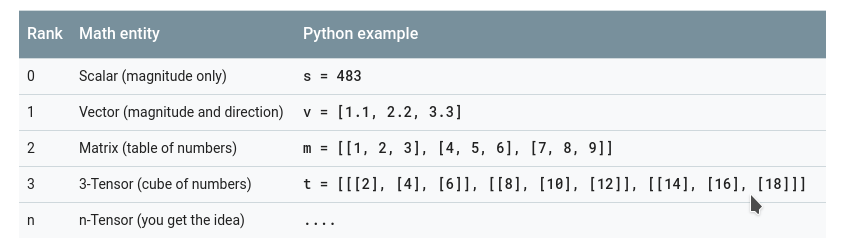
\includegraphics[width=0.8\textwidth]{img/rank.png}
    \caption{Rank}
    \label{fig:rank}
\end{figure}

\begin{figure}[h]
    \centering
    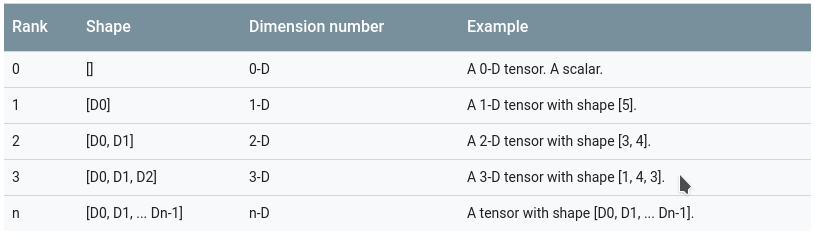
\includegraphics[width=0.8\textwidth]{img/shape.png}
    \caption{Shapes}
    \label{fig:shape}
\end{figure}


\subsection{Constants}
Constants is one type of tensor that has a value that does not change during runtime as in the case of the following example:

\begin{minted}{python}
node1 = tf.constant(3.0, dtype=tf.float32)
node2 = tf.constant(4.0) # also tf.float32 implicitly
\end{minted}

\subsection{Placeholders}
A graph can be parameterized to accept external inputs, known as placeholders. A placeholder is a tensor that usually receives a value before the execution of an TFG, as follow: 

\begin{minted}{python}
a = tf.placeholder(tf.float32)
b = tf.placeholder(tf.float32)
adder_node = a + b # + provides a shortcut for tf.add(a, b)

print(sess.run(adder_node, {a: 3, b: 4.5}))
print(sess.run(adder_node, {a: [1, 3], b: [2, 4]}))
\end{minted}


\subsection{Variables}
To make the model trainable, we need to be able to modify the graph to get new outputs with the same input. Variables is a type of tensor that allows us to add trainable parameters to a graph.
A variable is the best way to represent shared, persistent state manipulated by your program.

\begin{minted}{python}
W = tf.Variable([.3], dtype=tf.float32)
b = tf.Variable([-.3], dtype=tf.float32)
x = tf.placeholder(tf.float32)
linear_model = W * x + b
sess = tf.Session()
print(sess.run(linear_model, {x: [1, 2, 3, 4]}))
\end{minted}

\subsection{TensorFlow Graph}
A TensorFlow Graph is composed of operations arranged in a graph, where a node describes an operation and the edges represent tensors. The TensorFlow example below generate the TFG that is shown in Figure \ref{fig:tfg_ex}.

\begin{minted}{python}
X = tf.placeholder(tf.float32)
Y = tf.placeholder(tf.float32)
Constant = tf.constant(5, tf.float32)

add = tf.add(X,Y)
mult = tf.multiply(add, Constant)

session = tf.Session()
result = session.run(mult, feed_dict={X: [5,2,1] , Y: [10,6,1]})

\end{minted}
 

\begin{figure}[H]
    \centering
    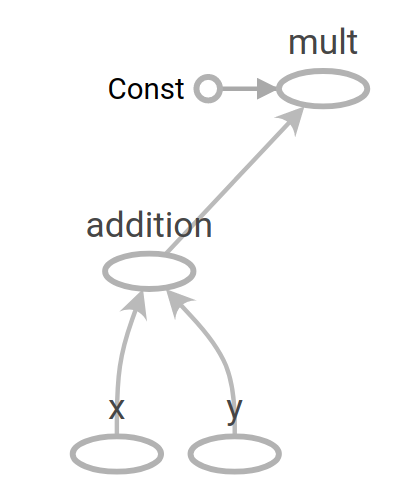
\includegraphics[width=0.2\textwidth]{img/tfg_example.png}
    \caption{TensorFlow Graph}
    \label{fig:tfg_ex}
\end{figure}


\subsection{TensorFlow Runtime}
The TensorFlow runtime sweeps all nodes in the TFG and executes each one of them according to the operation
that it describes (e.g. multiply). The user can use TensorFlow in several different languages (e.g. Python, Java). 

The Figure \ref{fig:tfg_runtime} shows the steps taken when executing a TensorFlow's program. 
First, given a TensorFlow code, it is converted into an TFG. After that, the TensorFlow runtime sweeps
this TFG executing each operation contained in it.  
Given a specific operation (e.g. Add) the Executor seeks at the available Kernels the most 
appropriate for the user's architecture.


\begin{figure}[H]
    \centering
    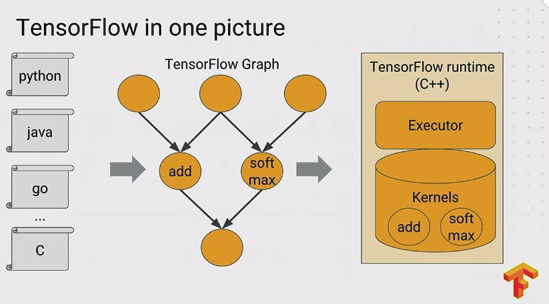
\includegraphics[width=0.7\textwidth]{img/tf_runtime.png}
    \caption{TensorFlow Runtime}
    \label{fig:tfg_runtime}
\end{figure}


\subsection{Device Placement}

The TensorFlow allows the user to choose the device where a given variable will be allocated as described below.

\begin{minted}{python}
with tf.device("/gpu:1"):
  v = tf.get_variable("v", [1])
\end{minted}

It is also possible to choose a given device (e.g. GPU) to performs a specific computation as shown below.

\begin{minted}{python}
with tf.device("/device:CPU:0"):
  # Operations created in this context will be pinned to the CPU.
  img = tf.decode_jpeg(tf.read_file("img.jpg"))

with tf.device("/device:GPU:0"):
  # Operations created in this context will be pinned to the GPU.
  result = tf.matmul(weights, img)
\end{minted}

\subsection{TensorBoard}
The computations that uses TensorFlow - like training a massive deep neural network - can be complex and confusing. To make it easier to understand, debug, and optimize TensorFlow programs, it is possible to use a suite of visualization tools called TensorBoard. It is possible to use TensorBoard to visualize the TensorFlow graph, plot quantitative metrics about the execution of your graph, and show additional data like images that pass through it.
 

\section{XLA}

XLA (Accelerated Linear Algebra) is a compiler for linear algebra that optimizes TensorFlow computations. XLA works with just-in-time (JIT) compilation or ahead-of-time (AOT) compilation, and the objectives are Improve execution speed, Improve memory usage, Reduce reliance on custom Ops , Reduce mobile footprint and Improve portability.

The optimization that improves the execution speed comes mainly by the ability of XLA to fuse operations. The TensorFlow runtime - without the XLA compilation, works by loading the inputs from the memory, perform the computation that uses it, and store the result into the memory before executing the next node in the TFG. Fuse computation means performing more than one node at the same time. For example, the piece of code below: 

\begin{minted}{C}
for(...) //Kernel 1
   A[i] = B[i] + C[i];

for(...) //Kernel 2
   D[i] = A[i] * B[i];
\end{minted} 

Can be converted into just:

\begin{minted}{C}
for(...) //Kernel 1 and Kernel 2 merged
   D[i] = (B[i] + C[i]) * B[i];
\end{minted} 

Besides the fact of fusing operations, which eliminates the necessity of loading from memory the input between the Kernel 1 and Kernel 2. It also reduces the memory usage - given that the array A will not be created after the optimization.

The diagram in Figure \ref{fig:xla_2} shows the entire execution when TensorFlow perfoms JIT or AOT. In the sequence the graph will be explained in details.

\begin{figure}[!htb]
    \centering
    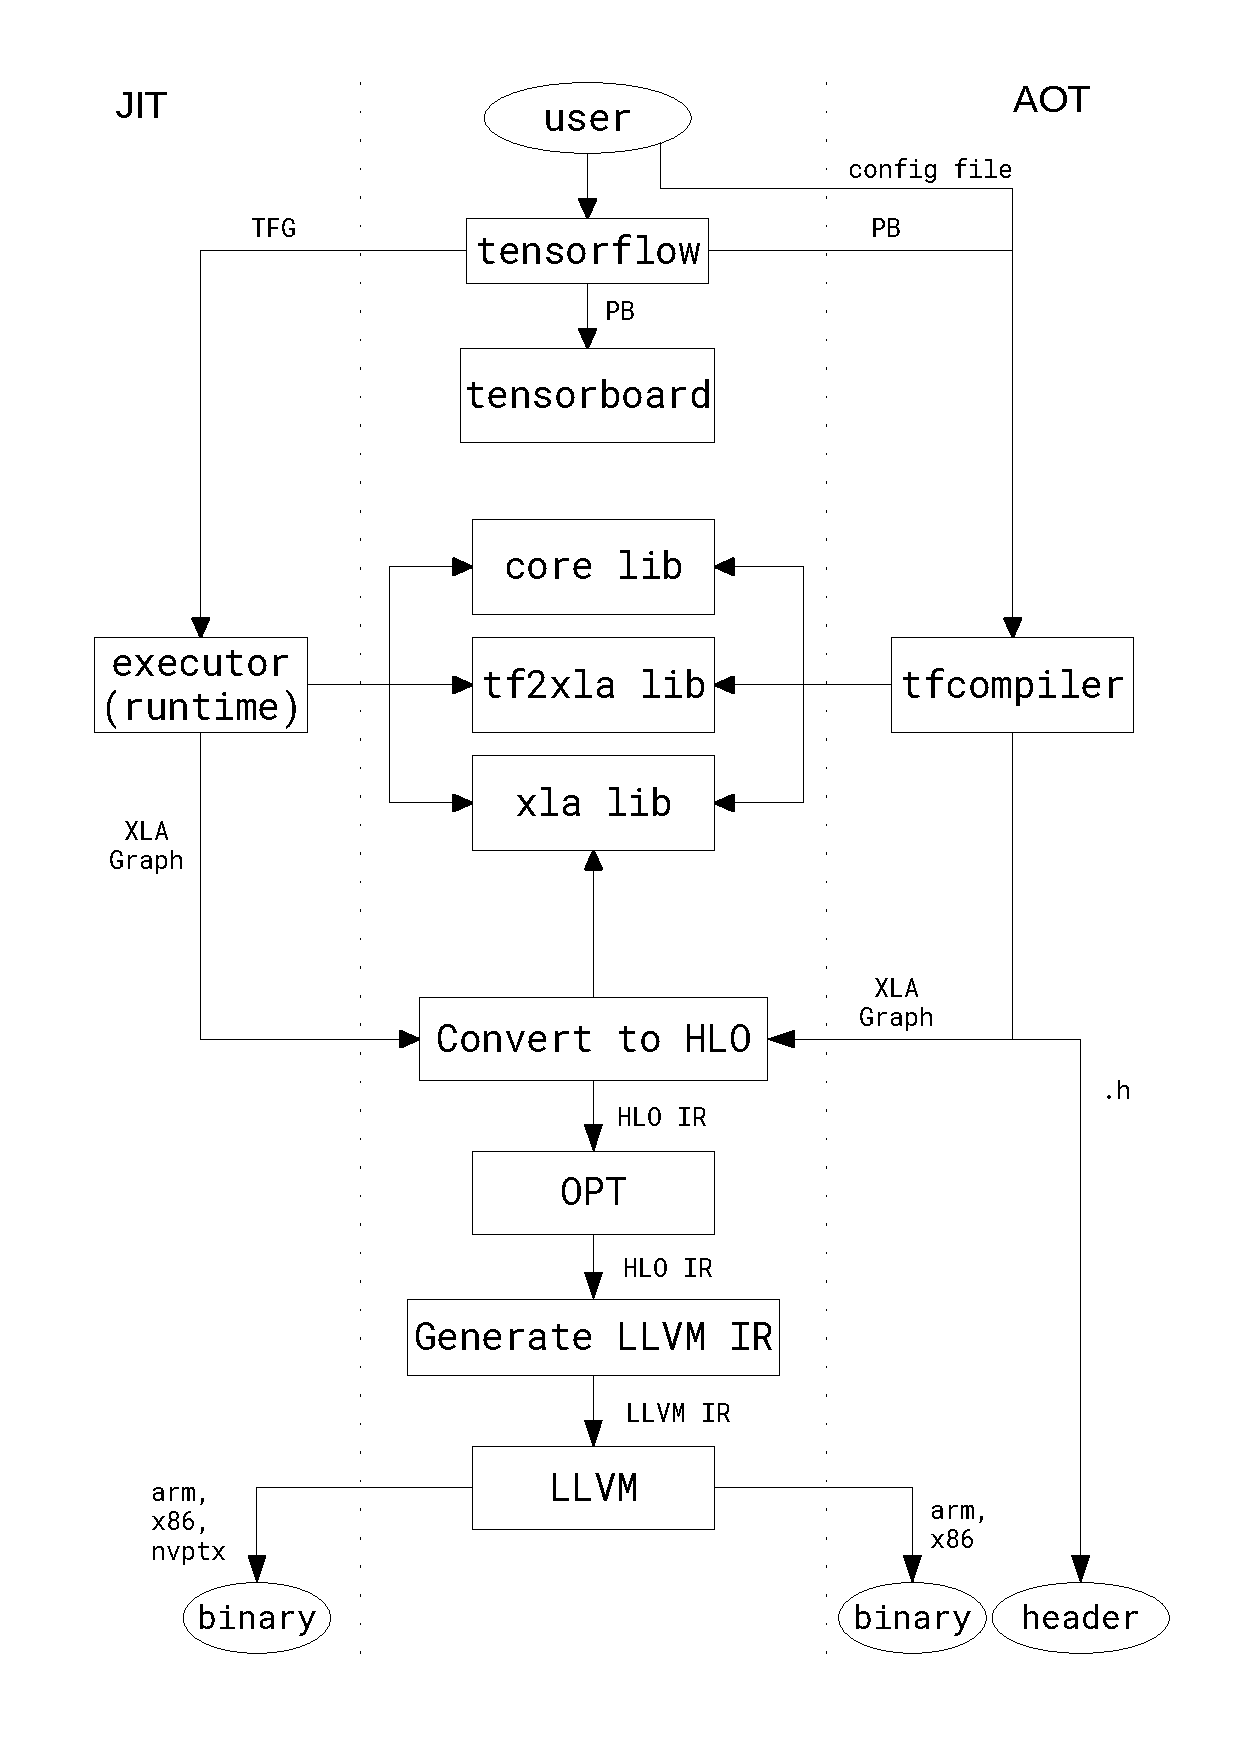
\includegraphics[width=0.7\textwidth]{flow/flow.pdf}
    \caption{TensorFlow execution with JIT and AOT}
    \label{fig:xla_2}
\end{figure}

From the code written by the user, the first step taken during the execution is the construction of the TFG. The persistent way to describe an TFG is by using the protobuf. The TFG is used to feed both JIT and HLO - by means of a protobuf file. 

The XLA, in summary, is composed of libraries that perform transformations, optimizations during  JIT and AOT executions. Those libraries are: core, xla and tf2xla.

The library core defines several features used by TensorFlow. Besides the data structures, common functions, protobuf definitions and others. The core is responsible to execute the TensorFlow runtime (executor).

The library xla, in general, is responsible to convert a given XLA Graph into binary. First, the XLA graph - also known as HLO IR, or just HLO (High Level Optimizer), is lowered to an LLVM IR in order to be compiled by the LLVM to a given binary of a specific architecture (e.g. x86), as shown in Figure \ref{fig:xla_xlalib}. 

The CPU and GPU back-ends included with XLA use LLVM for low-level IR, optimization, and code-generation. These back-ends emit the LLVM IR necessary to represent the XLA HLO computation in an efficient manner, and then invoke LLVM to emit native code from this LLVM IR.

\begin{figure}[h]
    \centering
    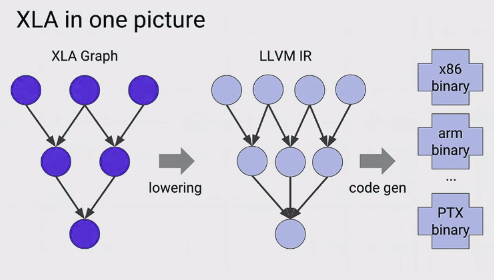
\includegraphics[width=0.7\textwidth]{img/xlalib.png}
    \caption{Library xla}
    \label{fig:xla_xlalib}
\end{figure}

The library tf2xla is responsible to convert an TFG into an XLA Graph. The Figure \ref{fig:xla_xlalib} shows it by converting the entire TensorFlow Graph into an XLA Graph. For instance, the node add - that performs the operation of addition, is converted to just one node at the XLA Graph. On the other hands, the softmax node in the XLA Graph is converted into three nodes in the XLA Graph. The conversion is done by means of a tf2xla kernels, that maintain all correspondents XLA nodes to a given TFG node. 

\begin{figure}[h]
    \centering
    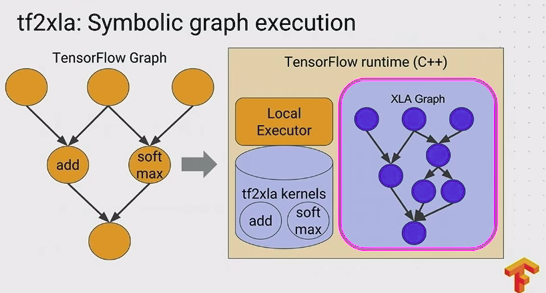
\includegraphics[width=0.7\textwidth]{img/tf2xlalib.png}
    \caption{Library tf2xla}
    \label{fig:xla_xlalib}
\end{figure}

The following sections describe in more details the flow taken by JIT and AOT according to the Figure \ref{fig:xla_2}.

\subsection{JIT Compilation}

The JIT compilation compiles and runs parts of TensorFlow graphs via XLA, it has the advantage of analyses and try to otmize to run several operation into a small number of compiled kernels, it means while Tensorflow runtime has to run each operation separately, the JIT can reduce memory bandwidth requirements and improve performance.

There are two ways to run TensorFlow computations via XLA, either by JIT-compiling operators placed on a CPU or GPU device, or by placing operators on the XLA\_CPU or XLA\_GPU TensorFlow devices. It means, when describing the graph on python interface, the user can specify if the JIT compile will be used, or the automatic way (session), that you specify that a session will use JIT, and XLA will decide which operation must be done using the JIT.

Turning on JIT compilation at the session level will result in all possible operators being greedily compiled into XLA computations. Each XLA computation will be compiled into one or more kernels for the underlying device. Follows an example of using that on python.

\begin{minted}{python}
# Config to turn on JIT compilation
config = tf.ConfigProto()
config.graph_options.optimizer_options.global_jit_level = tf.OptimizerOptions.ON_1
sess = tf.Session(config=config)
\end{minted}

In the manual mode you can decide which operation nodes must be done using JIT, for example:

\begin{minted}{python}
jit_scope = tf.contrib.compiler.jit.experimental_jit_scope
x = tf.placeholder(np.float32)
with jit_scope():
    y = tf.add(x, x)  # The "add" will be compiled with XLA.
\end{minted}


During the execution of a program with JIT (e.g. annotated to be compiled), the executor identify the node before its execution and identify if this module were compiled previously. If so, the compiled module is used and the execution continues to the next nodes in the TFG. Otherwise, the TFG is node is compiled into HLO IR, it passes into several optimizations, then it is transformed into an LLVM IR, and finally, it is compiled. The binary is executed and the runtime continues its execution, executing the following nodes.


The example in Figure \ref{fig:xla_jitex} shows how JIT works. First, it identifies the nodes to be compiled, then the nodes are compiled and executed.

\begin{figure}[h]
    \centering
    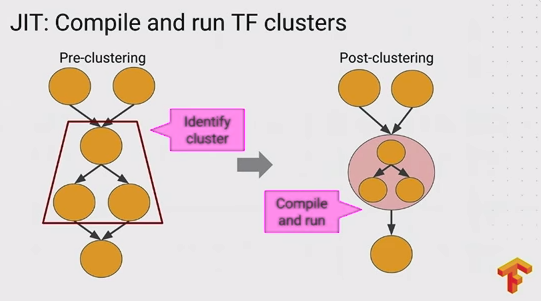
\includegraphics[width=0.68\textwidth]{img/jit_ex.png}
    \caption{JIT example}
    \label{fig:xla_jitex}
\end{figure}

\section{AOT compilation}

The TensorFlow graph is normally executed by the TensorFlow runtime. This incurs some runtime overhead for execution of each node in the graph. This also leads to a larger total binary size, since the code for the TensorFlow runtime needs to be available, in addition to the graph itself, the tfcompile can reduce total binary size, and also avoid some runtime overheads.

With those characteristics, AOT compilation can be considered one nice approach when using devices with few resources.

\subsection{tfcompile}

tfcompile implements ahead-of-time (AOT) compilation for TensorFlow graphs, it means, it compiles Tensorflow model into native machine code, tfcompile uses LLVM API to generate native code, and make some optimization, according to the Figure \ref{fig:xla_aotex}.

\begin{figure}[h]
    \centering
    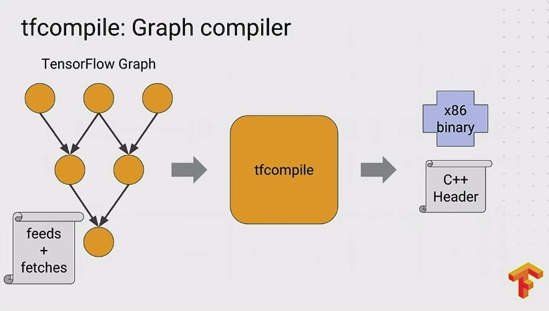
\includegraphics[width=0.68\textwidth]{img/aot_ex.png}
    \caption{AOT example}
    \label{fig:xla_aotex}
\end{figure}

In summary, it is necessary to pass to the tfcompiler the protobuf - file that contains the nodes of the TFG, and a config file containing the feeds and fetches - described below. With those files, the tfcompile generate the HLO IR, that is compiled by using the XLA infrastructure until the binary file. Besides that, the tfcompiler also generate an header file. The tfcompiler does not execute the TensorFlow model, it only generates the binary and header file that has to be linked in a program created by the user. 

For use the tfcompile you have to follow some steps:

\subsection{Configure the subgraph to compile}

Identify the feeds and fetches that correspond to the input and output arguments for the generated function. Then configure the feeds and fetches in a tensorflow.tfcompile.Config proto.

\begin{minted}{protobuf}
# Each feed is a positional input argument for the generated function.  The order
# of each entry matches the order of each input argument.  Here “x_hold” and “y_hold”
# refer to the names of placeholder nodes defined in the graph.
feed {
  id { node_name: "x_hold" }
  shape {
    dim { size: 2 }
    dim { size: 3 }
  }
}
feed {
  id { node_name: "y_hold" }
  shape {
    dim { size: 3 }
    dim { size: 2 }
  }
}

# Each fetch is a positional output argument for the generated function.  The order
# of each entry matches the order of each output argument.  Here “x_y_prod”
# refers to the name of a matmul node defined in the graph.
fetch {
  id { node_name: "x_y_prod" }
}
\end{minted}


\subsubsection{Use tf\_library build macro to compile the subgraph}

This part uses bazel to build the graph, it means, bazel gives to tfcompile the parameters of tensorflow model(pb file), and the file of feed and fetches (input and outputs) and tfcompile generate an ojbect file, .so, and a header file in C++.

\begin{minted}{python}
load("//third_party/tensorflow/compiler/aot:tfcompile.bzl", "tf_library")

# Use the tf_library macro to compile your graph into executable code.
tf_library(
    # name is used to generate the following underlying build rules:
    # <name>           : cc_library packaging the generated header and object files
    # <name>_test      : cc_test containing a simple test and benchmark
    # <name>_benchmark : cc_binary containing a stand-alone benchmark with minimal deps;
    #                    can be run on a mobile device
    name = "test_graph_tfmatmul",
    # cpp_class specifies the name of the generated C++ class, with namespaces allowed.
    # The class will be generated in the given namespace(s), or if no namespaces are
    # given, within the global namespace.
    cpp_class = "foo::bar::MatMulComp",
    # graph is the input GraphDef proto, by default expected in binary format.  To
    # use the text format instead, just use the ‘.pbtxt’ suffix.  A subgraph will be
    # created from this input graph, with feeds as inputs and fetches as outputs.
    # No Placeholder or Variable ops may exist in this subgraph.
    graph = "test_graph_tfmatmul.pb",
    # config is the input Config proto, by default expected in binary format.  To
    # use the text format instead, use the ‘.pbtxt’ suffix.  This is where the
    # feeds and fetches were specified above, in the previous step.
    config = "test_graph_tfmatmul.config.pbtxt",
)
\end{minted}

tfcompile cannot compile variables and placeholders, so you must use the freezegraph script to convert variables in constants, this variables is not the input variables, it is the parameters of your network, the inputs must be specified in tfcompile.Config file.

\subsection{Invoke the subgraph}

After build with bazel, an object file and a header file is generate to use with C++, in this example, the C++ header has the follow format:

\begin{minted}{c++}

namespace foo {
namespace bar {

// MatMulComp represents a computation previously specified in a
// TensorFlow graph, now compiled into executable code.
class MatMulComp {
 public:
  // AllocMode controls the buffer allocation mode.
  enum class AllocMode {
    ARGS_RESULTS_AND_TEMPS,  // Allocate arg, result and temp buffers
    RESULTS_AND_TEMPS_ONLY,  // Only allocate result and temp buffers
  };

  MatMulComp(AllocMode mode = AllocMode::ARGS_RESULTS_AND_TEMPS);
  ~MatMulComp();

  // Runs the computation, with inputs read from arg buffers, and outputs
  // written to result buffers. Returns true on success and false on failure.
  bool Run();

  // Arg methods for managing input buffers. Buffers are in row-major order.
  // There is a set of methods for each positional argument.
  void** args();
  void set_arg0_data(float* data);
  float* arg0_data();
  float& arg0(size_t dim0, size_t dim1);
  void set_arg1_data(float* data);
  float* arg1_data();
  float& arg1(size_t dim0, size_t dim1);

  // Result methods for managing output buffers. Buffers are in row-major order.
  // Must only be called after a successful Run call. There is a set of methods
  // for each positional result.
  void** results();
  float* result0_data();
  float& result0(size_t dim0, size_t dim1);
};

}  // end namespace bar
}  // end namespace foo
\end{minted}

Where set\_arg0\_data and set\_arg1\_data are used to give the input, so you must run and get the result with result0\_data, the dimension is according what was passed in config file.

Follows an example to use the files generated by tfcompile:

\begin{minted}{c++}
#define EIGEN_USE_THREADS
#define EIGEN_USE_CUSTOM_THREAD_POOL

#include <iostream>
#include "third_party/eigen3/unsupported/Eigen/CXX11/Tensor"
#include "tensorflow/compiler/aot/tests/test_graph_tfmatmul.h" // generated

int main(int argc, char** argv) {
  Eigen::ThreadPool tp(2);  // Size the thread pool as appropriate.
  Eigen::ThreadPoolDevice device(&tp, tp.NumThreads());

  foo::bar::MatMulComp matmul;
  matmul.set_thread_pool(&device);

  // Set up args and run the computation.
  const float args[12] = {1, 2, 3, 4, 5, 6, 7, 8, 9, 10, 11, 12};
  std::copy(args + 0, args + 6, matmul.arg0_data());
  std::copy(args + 6, args + 12, matmul.arg1_data());
  matmul.Run();

  // Check result
  if (matmul.result0(0, 0) == 58) {
    std::cout << "Success" << std::endl;
  } else {
    std::cout << "Failed. Expected value 58 at 0,0. Got:"
              << matmul.result0(0, 0) << std::endl;
  }

  return 0;
}
\end{minted}

\end{document}
